\chapter{提案手法/アルゴリズム} \label{chp:2}
\section{検討}
本節は容器に液体を定量的に注ぐ方法について，検討する．
研究目的に書いた通り，本研究では主な2つの課題とそれ以外の3つの課題が含む．
本節は主な2つの課題について説明する．
それ以外の3つの部分は第四章:手法の実装で説明する．

	\subsection{体積の計算方法}
	本項は注ぎ作業における通用な体積の計算方法について説明する．
	
	研究目的1(注いだ体積を計測すること)を実現する方法は，体積を計算する方法(例えば，力覚センサ、計量コップ、秤やビュレットなど)により，多数ある．
	そして，\ref{sec:Intro}節の注ぎ作業の考察により，料理ロボットにおける体積を計算する方法は容器モデルの積分による方法と考えた．
	
	この方法は容器のモデルを視覚センサで計測し，そのモデルを積分することで，複雑な形状の体積が計算できる．
	
	\subsection{注ぐ手法}
	体積の計算方法は容器モデルによる方法を使用し，注いだ体積の測り方は，注ぐ容器に注目する方法と，注ぎ先容器に注目する方法の2つの方法を考えた．
	
		\subsubsection{手法1：注ぎ先容器に注目する}\label{sec:pour-method1}
		手法1は注ぎ先容器に注いだ液体の液面高さに注目し，注ぐ時に液面高さを注いだ体積にリアルタイムに計算し，注ぐ容器の傾き角速度を操作量，注いだ体積を制御量とするPD制御で注ぎ作業を実現する手法である．
		
		料理によく使われる液体調味料(酢や醤油や油など)は流動性が高い液体だと考えられる．
		流動性が高い液体において，大きな外力がないなら，液面が常に水平面と平行する．% 日本語問題:水平面は正しいですか？
		その特性を利用し，注ぎ先容器モデルの底から液面まで間の体積を注いだ液体の体積とする．
		そして，液面高さと容器のモデルが分かれば，底から液面の間の体積，つまり注いだ液体の体積が計算できるはずである．
		
		しかし，注ぎ作業を実現することには，注いだ体積を正確に計測することだけではできない．
		目標体積になるまで，正確に注ぐためにロボットを制御することも必要である．
		
		そこで，手法1における，制御の方法は，目標体積と注いだ体積の差を誤差とし，注ぐ容器の傾き角速度を制御量とするPD制御を用いる．
		なぜなら，手法1は注ぐ容器のモデル化が困難で，注いだ体積と注ぐ容器の傾き角度の関係が計算できない場合において，PD制御は確実に注いだ液体を目標体積に到達させる方法だからである．
				
		この手法の利点は注ぐ容器の状態や形状がわからなくても，正確に注げることである．
		一方，注ぎ先の容器の形状が計測できないなら使えなくなる．
		
		\subsubsection{手法2：注ぐ容器を注目する}\label{sec:pour-method2}
		手法1の欠点を解決するため，注ぎ先の容器に注目することをやめ，注ぐ容器に注目する．
		手法2は注ぐ容器モデルと注ぐ容器の初期液体の体積を計測し，注いだ体積と注ぐ容器の傾き角度の関係により，注ぐ容器を目標体積に対応する傾き角度に傾けることで注ぎ作業を実現する手法である．
		
		具体的には，
		まず，注ぐ容器において2つ条件がある:
		\begin{enumerate}
			\item 注いでいる時，液面高さと注ぎ口の最低点の高さが同じである．
			\item 注ぎ作業において，注ぎ先容器が溢れない限り，注ぐ容器から出た体積は必ず注いだ体積である．
		\end{enumerate}
		この2つ条件により，注ぐ容器の初期液体体積と注ぐ容器のモデルが分かれば，注いだ体積と注ぐ容器の傾き角度の関係が計算できる．
		その関係により，注ぐ容器を目標体積に対応する傾き角度に傾ければ，目標体積の液体が出る．
		
		手法1と同じように，ロボットの制御が必要である．
		そこで，手法2は目標体積に対応する傾き角度が計算できるため，制御する方法はロボットアームをP制御で注ぐ容器をその角度に傾ける．
		
		手法2は手法1の欠点が解決できる一方，注ぐ容器の形状と初期液体体積が計測できないなら使えなくなる．
			
		\subsubsection{注ぐ手法のまとめ}
		手法1は注ぎ先の容器に注いだ液体の液面高さを見，注ぐ容器の傾き角速度のPD制御をすることにより，注ぎ作業を達成する手法である．
		
		手法2は注ぐ容器の形状と初期液体体積を計測し，注いだ体積と注ぐ容器の傾き角度の関係を計算し，目標体積に対応する傾き角度に注ぐ容器を回転させることにより，注ぎ作業を達成する手法である．
		%TODO:添加对比表格
		
		2つ手法を合わせ，注ぐ容器か注ぎ先容器かどちらかが計測できれば，注いだ体積の測定が可能になる．
		そして，各手法に対応する注ぎ動作の制御を合わせて，最終的に液体を定量的に注ぐことを実現する．

\section{体積の計算}\label{sec:LiquidVolume}
本節は，液体を注ぐ手法の検討による体積の計算方法の詳細について説明する．

ここでは，任意の容器のある傾き角度$\theta$に対して，底からある高さ$H$までの体積(つまり図\ref{fig:ParametersV4}青い部分)を計算する．

\begin{figure}[h]
	\centering
	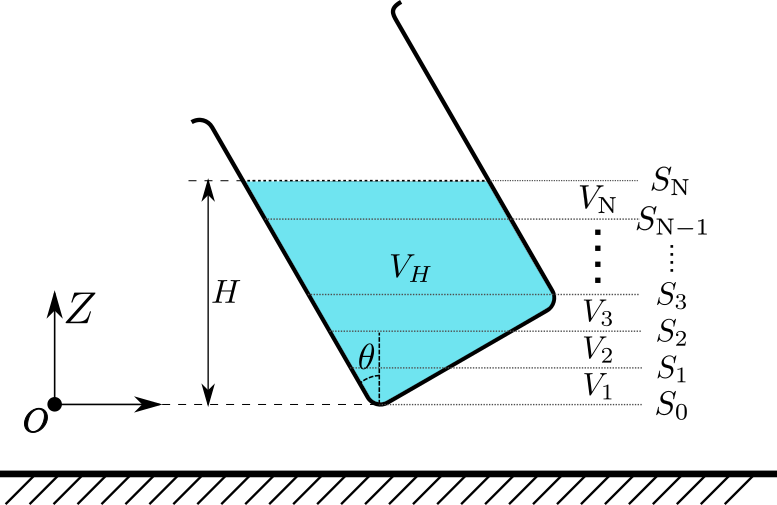
\includegraphics[width=.6\linewidth]{fig/chp2/ParametersV4.png}
	\caption{パラメータの説明}
	\label{fig:ParametersV4}
\end{figure}

あらかじめ容器のモデルが得られているとする．
そして，$V_H$の部分の体積は以下の式で決める：%傾き角度を$\theta$において，
$$V_{H,\theta}=\int_{0}^{H} S(h,\theta)dh$$
ここで，$S(h,\theta)$はある傾き角度$\theta$において，容器のモデルを高さ$h$の水平面で切る断面積である．
また，$S(h,\theta)$も$\theta$と$h$を変数とする容器のモデル関数である．

次に，上式の積分を計算するため，容器のモデルを複数の部分に分割し，各部分の体積の和を計算する．
z軸に沿ってそのモデルをある高さ$H$の間で${N}$個の部分に分割する．
各部分の高さを
$$ h_\mathrm{\delta}　= \frac{H}{{N}}$$
とおき，$n$番目の部分の体積$V_n$を以下の式で近似する．
$$V_n \approx \frac {(S_{n-1} + S_{n})\,h_\mathrm{\delta}}{2} \quad (n=1,2,3,\dots,{N})$$
ここで$S_{n-1}$は$n$番目の部分の下断面の面積であり，$S_{n}$は$n$番目の部分の上断面の面積である．
上の$S(h,\theta)$の定義により，以下の式を満たす：
$$S_n=S(h_\mathrm{\delta} \cdot n,\theta)$$

${N}$個の体積を全て足し合わせることで，上式の積分，つまり底からある高さ$H$までの体積$V_{H,\theta}$が以下のように計算される．
\begin{equation}
V_{H,\theta} = \int_{0}^{H} S(h,\theta)dh = \sum^{{N}}_{n=1} V_n 
\end{equation}
		
\section{手法1：注ぐ容器に注目する}	\label{sec:Method1}
本節は手法1のアルゴリズムの詳細を述べる．
	\subsection{液面高さに基づく注いだ体積の計算}\label{sec:Method1-liquidHeight}
	本項は\ref{sec:pour-method2}項で述べた，注ぐ時に液面高さを注いだ体積を計算する方法の詳細について説明する．
	
	注ぎ先容器の傾き角度$\theta$は注いでいる間で変わらないと仮定する．
	\ref{sec:pour-method1}項により，手法1はある傾き角度$\theta$に対して，底からある液面高さ$h_\mathrm{liquid,\theta}$の間の体積$V_\mathrm{liquid,\theta}$を注いだ体積$V_\mathrm{pour,\theta}$とする．
	\ref{sec:LiquidVolume}項により，$V_\mathrm{pour}$は以下の式を満たす：
	$$V_\mathrm{pour,\theta} = V_\mathrm{liquid,\theta} 
	= \int_{0}^{h_\mathrm{liquid}} S(h,\theta)dh $$
	この積分は\ref{sec:LiquidVolume}項の部分と同様に計算する．
	
	\subsection{注ぎ動作のPD制御}
	ここでは\ref{sec:Method1-liquidHeight}と\ref{sec:LiquidVolume}項の方法により計算した注いだ体積に基づいて，目標容器に目標体積の液体を入れる動作を生成する手法について述べる．
	注ぎ動作は，考察に書いた「傾きの制御」のほか，
	さらに「戻し動作」を加えた二つの部分からなる．
	
		\subsubsection{注ぐ時の傾き制御}
		傾きの制御は，
		注ぐ容器のモデルが未知の場合，注いだ体積と注ぐ容器の傾き角度の関係が計算困難であるため，初期状態(図\ref{fig:PD-Control}の半透明の部分)から手先座標系を注ぐ容器の注ぎ口に設定し(図\ref{fig:PD-Control}の薄いオレンジの座標系)，その傾き角速度をPD制御することで行う．
		なお，I制御が含まれていると，目標値に達しても積分項が注ぎ作業を続ける方向に働いてしまう．
		注ぎ作業では一度注いだ液体を元の容器に戻せないため，これは誤差の原因となってしまう．
		そのため，今手法はI制御を使用しない．
		
		操作量である傾き角速度$\omega$は，現在の体積$V_\mathrm{now}$と目標体積$V_\mathrm{tar}$の差$V_\mathrm{error}$の比例，微分（＝体積増加速度）$D_\mathrm{error}$で以下のように決める．
		$$ \omega = k_\mathrm{p}  V_\mathrm{error} + k_\mathrm{d}  D_\mathrm{error}$$
		誤差$V_\mathrm{error}$が大きい場合，上式の$\omega$をそのまま使うと，一気に大量の液体が注がれてしまう可能性があるため，$\omega$の値に上限と下限を設定した．具体的には，$-2^\circ/\mathrm{s} \leq \omega \leq 2^\circ/\mathrm{s}$の範囲を超えた場合は，この範囲を超えない最も近い値に$\omega$を設定する．% sとは何でしょうか？
		注ぎ動作の終了条件は$V_\mathrm{error} \leq 0$で，到達した後すぐに戻し動作を実行する．
		\begin{figure}[h]
			\centering
			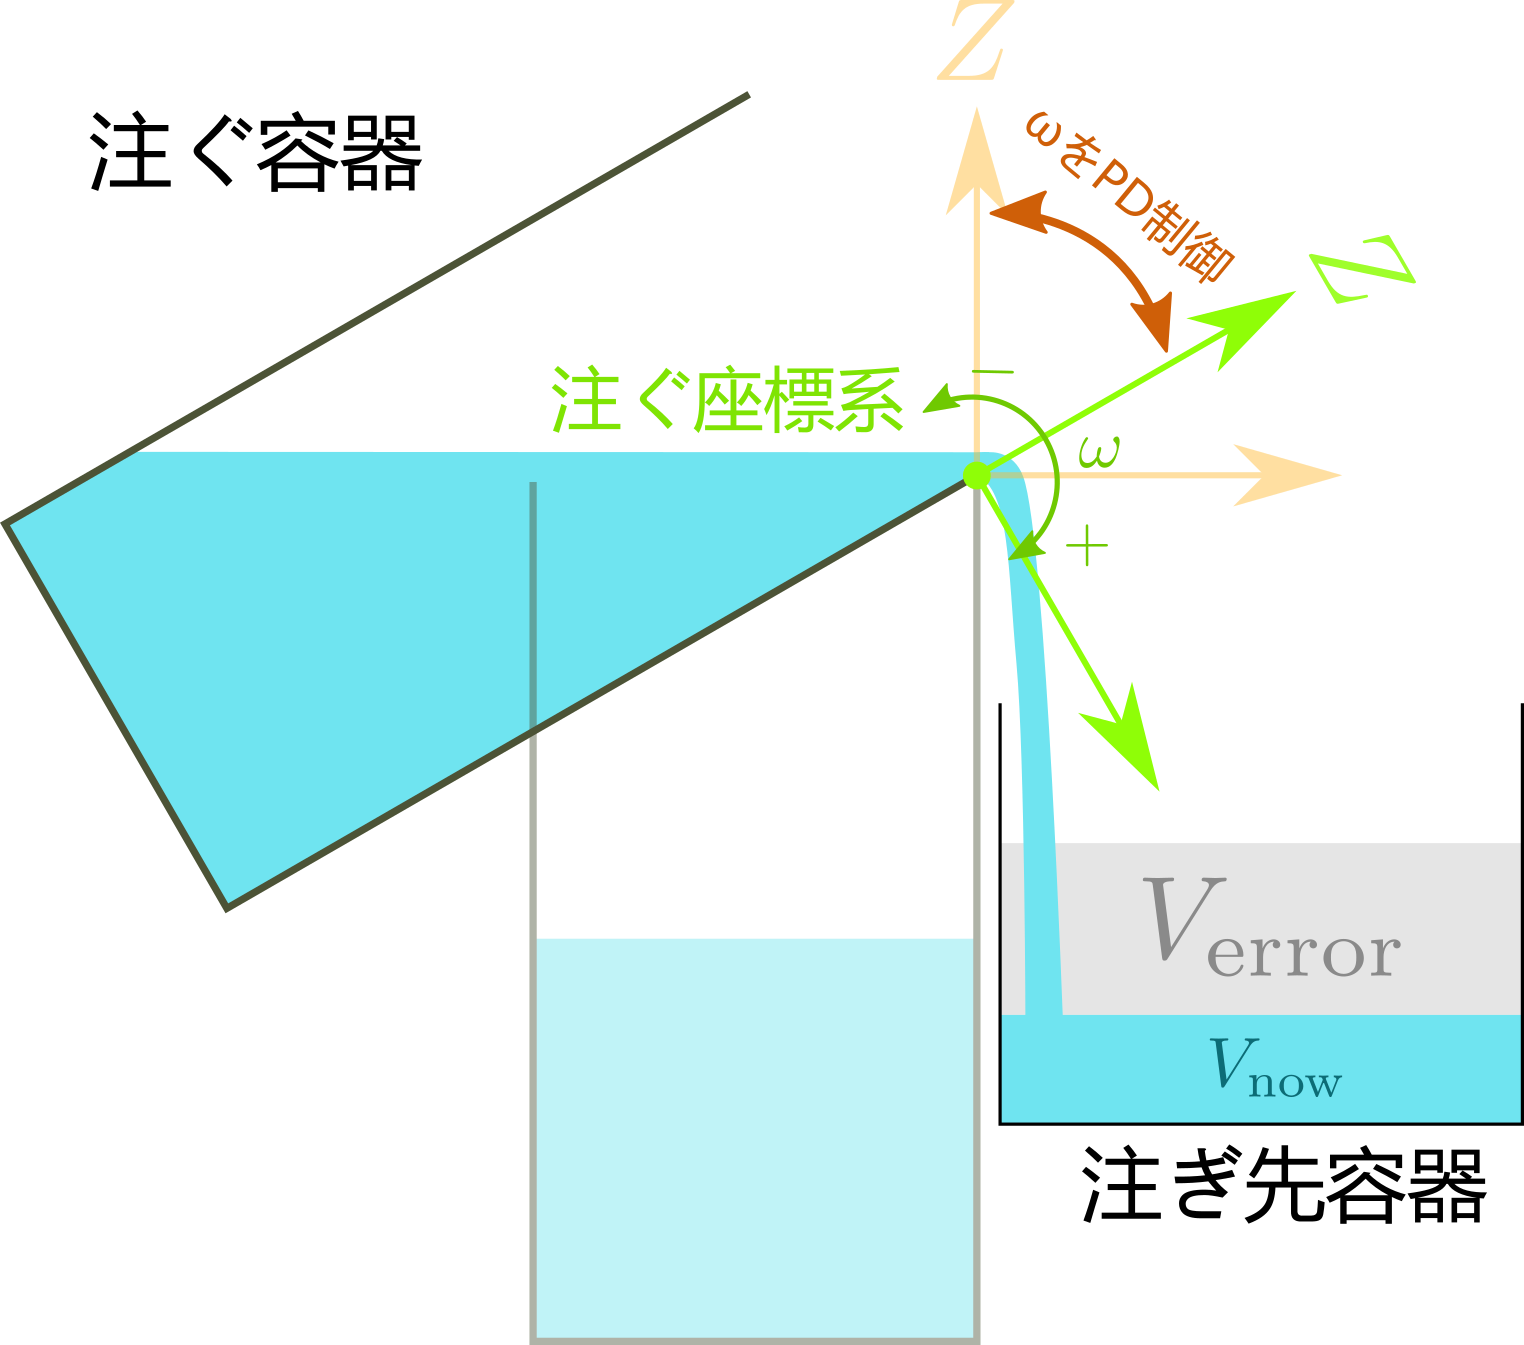
\includegraphics[width=0.65\linewidth]{fig/chp2/pourAction}
			\caption{PD制御の説明}
			\label{fig:PD-Control}
		\end{figure}
		
		\subsubsection{戻し動作}\label{sec:ReturnAction}
		戻し動作の目的は，目標体積に到達した後に液体の増加を出来る限り早く止めることである．具体的な動作は，PDコントローラを停止し(注ぐ容器は図\ref{fig:ReturnMotion}の半透明の状態)，手先座標系を戻し動作座標系(図\ref{fig:ReturnMotion}のピンクの座標系)に設定し，$\omega$の負の方向に，テーブルに対して垂直になるまで(図\ref{fig:ReturnMotion}のオレンジの状態)手先座標系を回転させる．
		\begin{figure}[h]
			\centering
			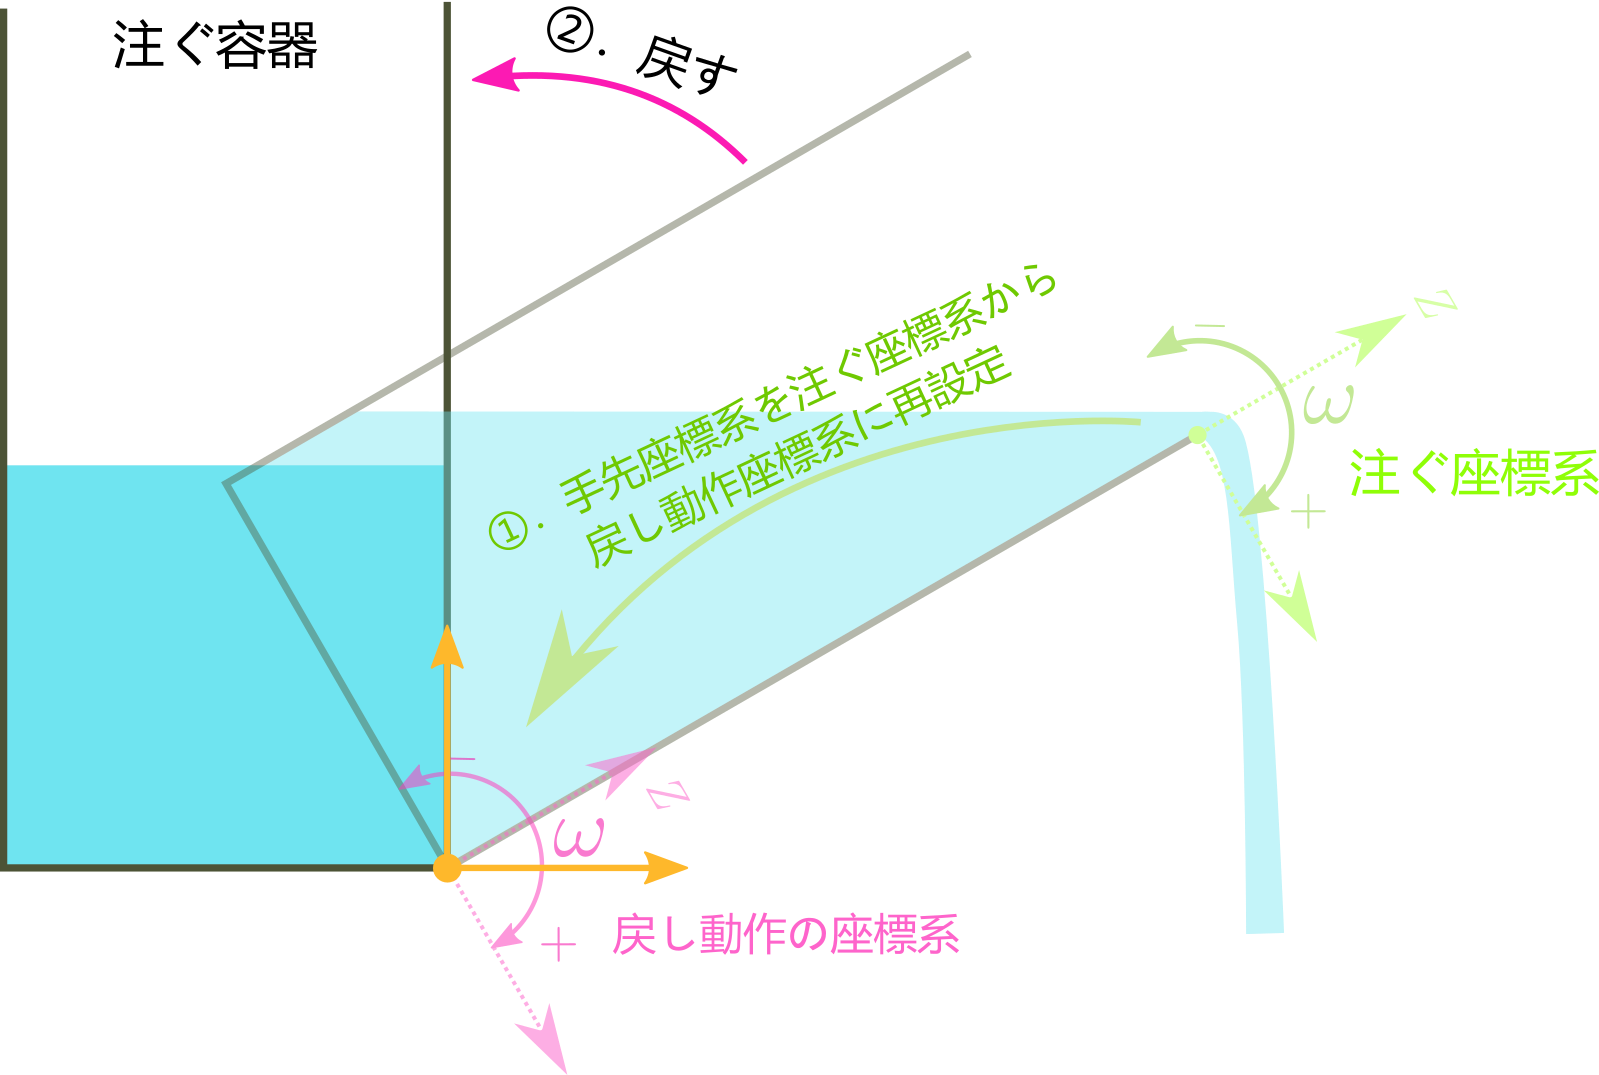
\includegraphics[width=0.65\linewidth]{fig/chp2/returnAction}
			\caption{戻し動作の説明}
			\label{fig:ReturnMotion}
		\end{figure}
	
\section{手法2：注ぎ先容器に注目する}	\label{sec:Method2}
	\subsection{注ぎ出した体積と注ぐ容器の傾き角度の関係による注いだ体積の計算}\label{sec:angle-and-volume}
	本項は，手法2における注いだ体積の計算について説明する．
	
	注ぐ容器のモデルと初期液体体積$V_\mathrm{init}$がすでに分かっていると仮定する．
	注ぎ前の時，注ぐ容器の傾き$\theta$に対して，
	\begin{figure}[h]
		\centering
		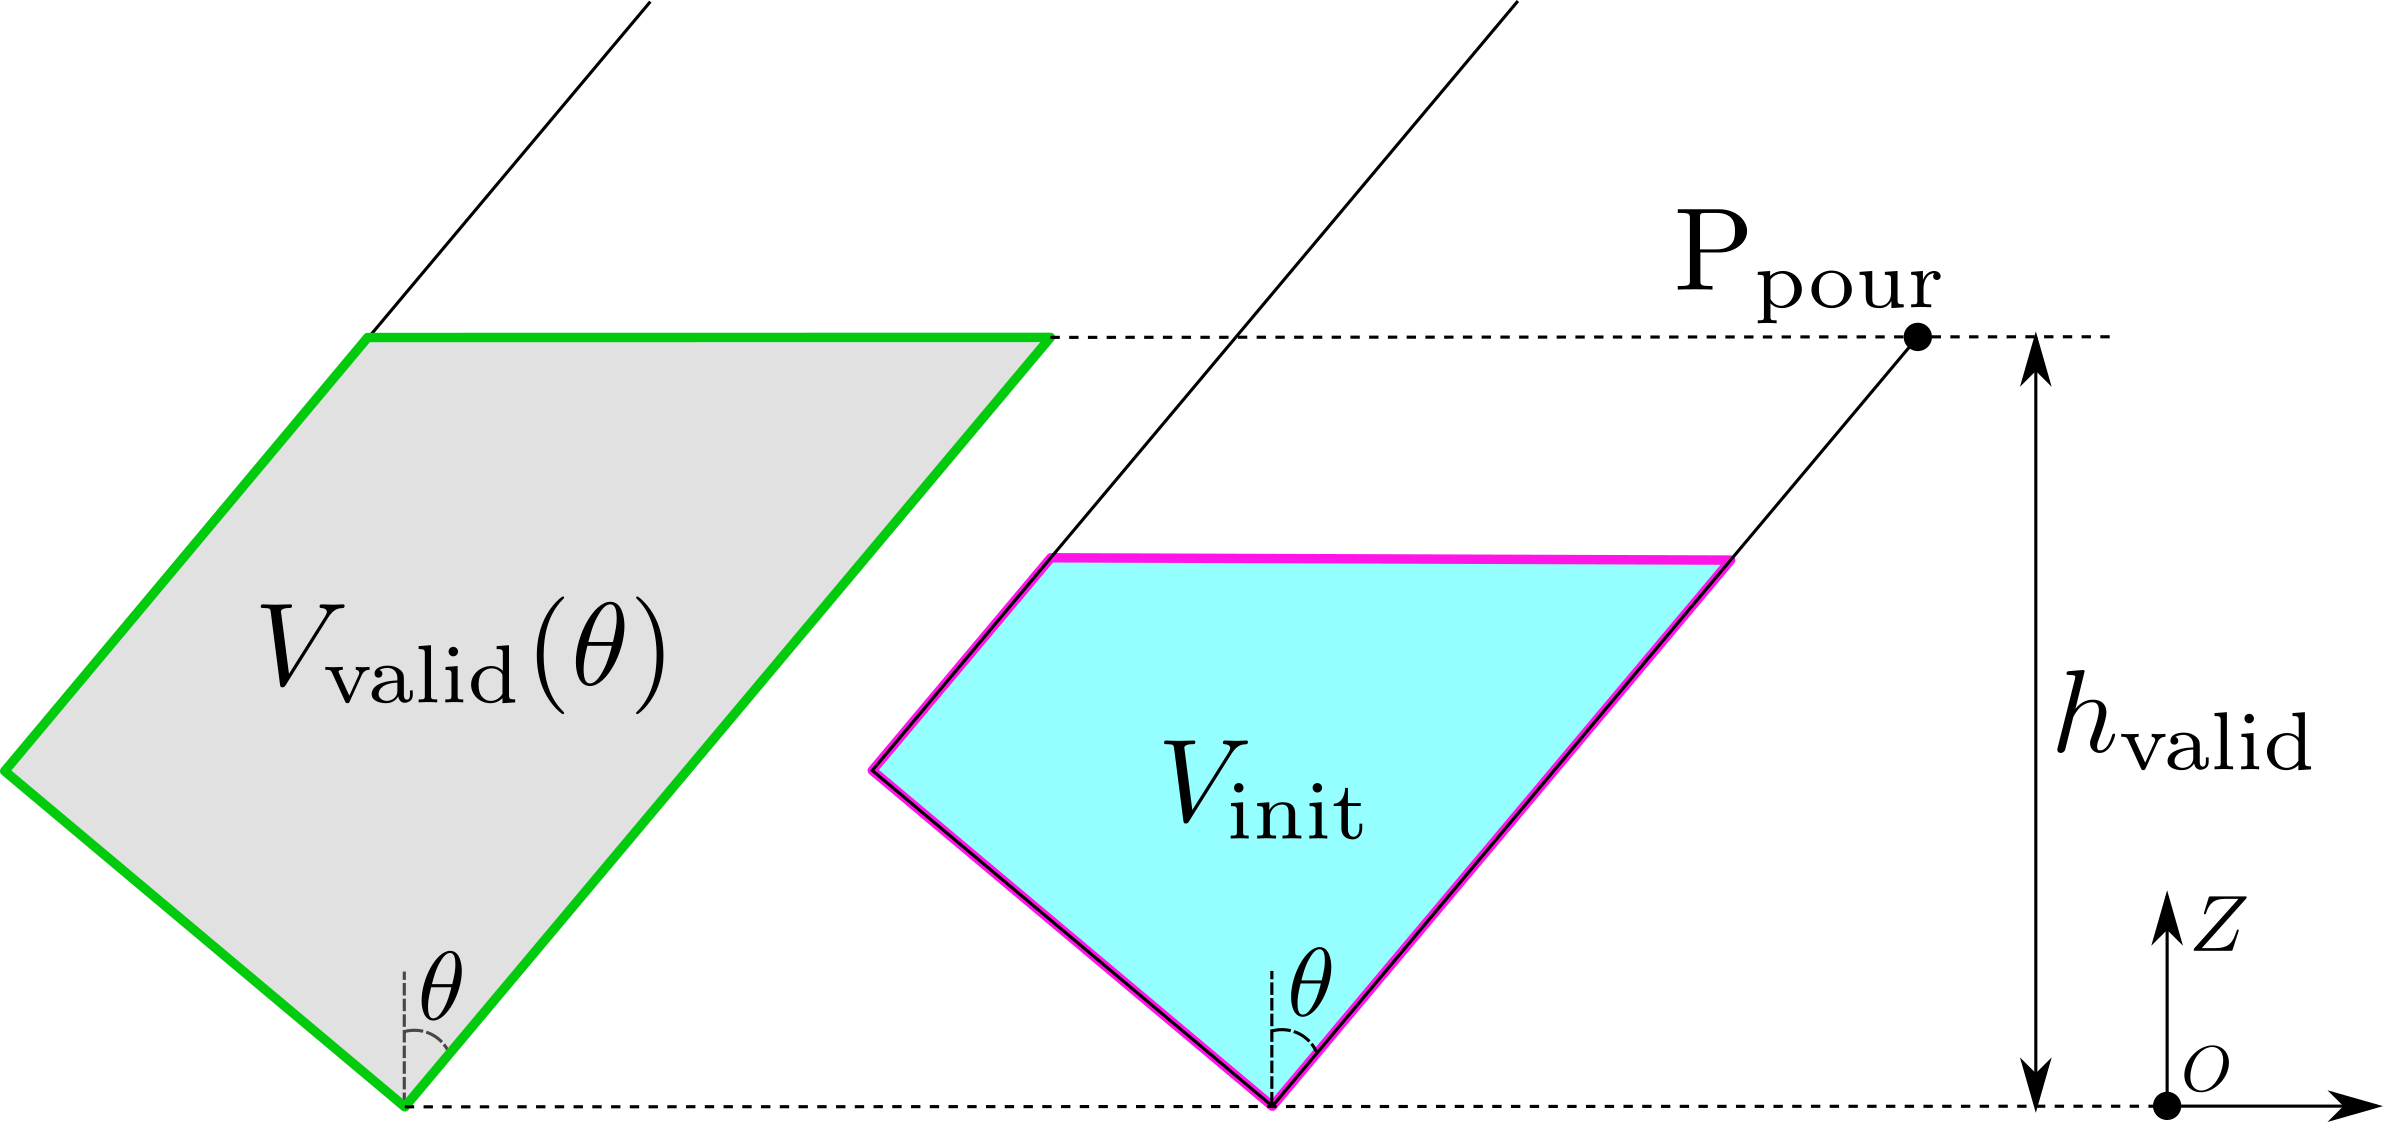
\includegraphics[width=0.7\linewidth]{fig/chp2/PourInit}
		\caption{注ぎ前の注ぐ容器}
		\label{fig:PourInit}
	\end{figure}
	%
	注ぎ縁の高さ$h_\mathrm{valid}(\theta)$を注ぐポイント$\mathrm{P}_\mathrm{pour}$とモデルの一番低い点のz軸に沿った距離として定める．
	$h_\mathrm{valid}(\theta)$は$\theta$に関する関数である．
	図\ref{fig:PourInit}のように，$V_\mathrm{valid}(\theta)$は現在の容器の傾き角度$\theta$においてこの容器の最大容積である(緑の枠)．
	$V_\mathrm{init}$は注ぐ容器の初期液体体積である(紫の枠)．
	そして，\ref{sec:LiquidVolume}項の方法により，$V_\mathrm{valid}(\theta)$の計算は以下の式で決める：

	$$V_\mathrm{valid}(\theta)=\int_{0}^{h_\mathrm{valid}(\theta)} S(h,\theta)dh$$
	この積分は\ref{sec:LiquidVolume}項と同様の計算をする．
	$h_\mathrm{valid}(\theta)$は次の\ref{sec:pour-point-detect}項を参照する．
	
	次に注ぎ動作中のある時点において，各変数の関係を説明する．図\ref{fig:Pouring}のように：% 文章が途切れてしまっています．
	\begin{figure}[h]
		\centering
		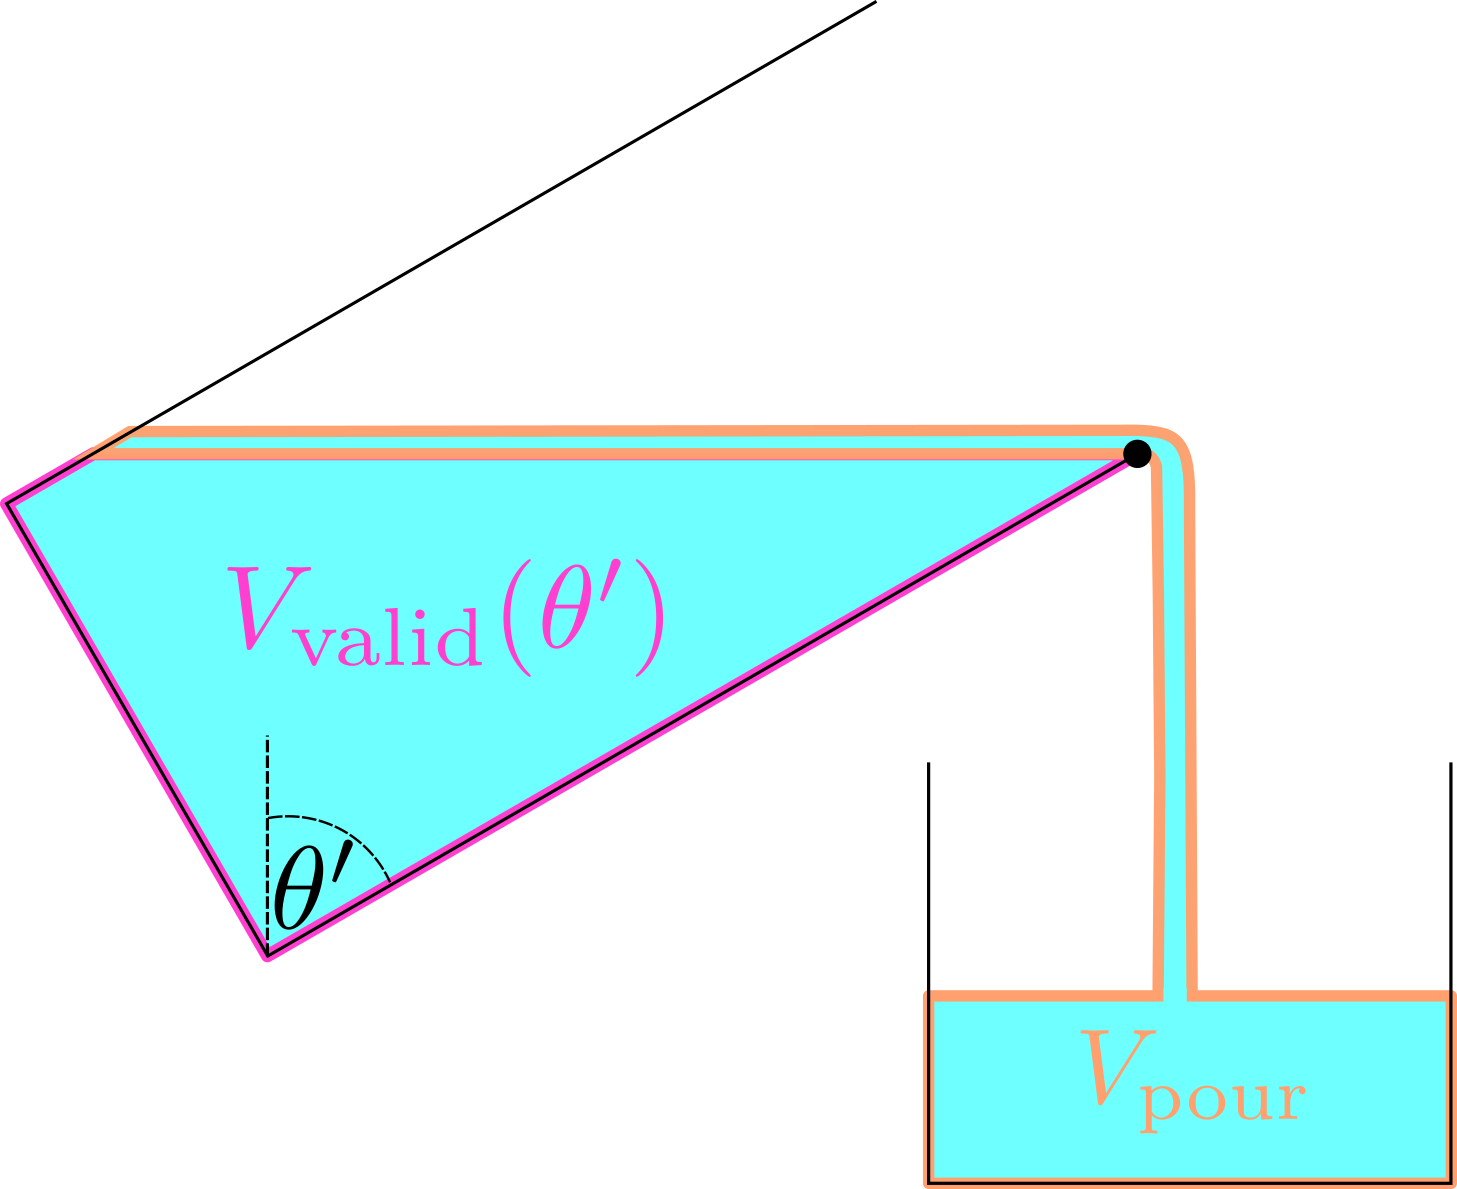
\includegraphics[width=0.6\linewidth]{fig/chp2/Pouring} % TODO :紫の部分の上側の線が見えません．
		\caption{注いでいる時の注ぐ容器}
		\label{fig:Pouring}
	\end{figure}

	$V_\mathrm{pour}$は注いだ液体の体積である(オレンジの枠)．
	$\theta^{\prime}$は注ぎ動作中のある時点における注ぐ容器の傾き角度である．
	注いでいる間は$V_\mathrm{valid}(\theta^{\prime})$(紫の枠の部分)は常に残した液体の体積$V_\mathrm{rest}$と同じである．
	つまり：
	$$V_\mathrm{valid}(\theta^{\prime})=V_\mathrm{rest}$$

	そして，\ref{sec:pour-method2}の2つ条件により,$V_\mathrm{init}$，$V_\mathrm{rest}$，$V_\mathrm{pour}$と$V_\mathrm{valid}(\theta^{\prime}節)$の関係は以下の式を満たす：
	\begin{equation}
	\begin{split}
	V_\mathrm{init}&=V_\mathrm{rest} + V_\mathrm{pour}\\
	&=V_\mathrm{valid}(\theta^{\prime}) + V_\mathrm{pour}
	\end{split}
	\end{equation}
	
	最後に，出す量と傾き角度$\theta$の関係$V_\mathrm{pour}(\theta)$は以下の式で決める．
	\begin{equation}
	V_\mathrm{pour}(\theta) = \left\{
	\begin{array}{lc}
	0 & if \quad V_\mathrm{valid}(\theta) > V_\mathrm{init}\\
	V_\mathrm{init} - V_\mathrm{valid}(\theta) & Otherwise
	\end{array}
	\right. 
	0\deg \leq \theta \leq 180\deg
	\end{equation}


	\subsection{注ぐポイントの検出}\label{sec:pour-point-detect}
	\ref{sec:angle-and-volume}により，出す量と傾き角度の関係の計算を実現するためには，注ぐポイント$\mathrm{P}_\mathrm{pour}節$の検出が必要である．
	注ぐポイントの定義は注ぎ縁の最低点である．
	本項は，それを検出するための「注ぎ縁の検出」と「注ぐポイントの検出」の2つの部分からなる．
	%TODO:用数学语言来表述。
	
		\subsubsection{注ぎ縁の検出}\label{sec:pour-edge-detect}
		注ぎ縁は容器の内部から外側に到達する縁である．
		したがって，容器をスライスすれば，注ぎ縁が入るスライスは必ず不連続な断線がある．
		それを利用し，同じ容器の様々な姿勢において，鉛直方向のスライスで，不連続な断線の端点が探せ，集めれば，注ぎ縁が検出できる．	
		%日本語問題：「断線の端点」より分かりやすい表現はありますか？
		
		\subsubsection{注ぐポイントの検出}
		注ぎ縁を抽出し，ある注ぐ方向に対して，注ぎ縁の最低点を探せば，注ぐポイントが検出できる．
		
	\subsection{注ぎ動作のP制御}
		\subsubsection{注ぐ時の傾き制御}
		手法2の制御は容器の注ぎ方向の傾き角速度を制御量とするP制御である．
		
		注ぐ容器と注ぎ先の容器がぶつからないように，手法1(\ref{sec:Method1}節)と同じ，ロボットの手先座標系を注ぐポイントに設定する．
		\ref{sec:angle-and-volume}の方法で，目標角度$\theta_\mathrm{tar}節$はすでに計算されたため，注ぎ動作の制御は単に容器を注ぎ方向の傾き角度に傾ければ良い．
		
		具体的には：
		現在の傾き角度$\theta$と目標値である目標角度$\theta_\mathrm{tar}$の差をP制御の誤差$\theta_\mathrm{error}$とする．
		そして，制御量である傾き角速度$\omega$は以下の式を満たす：
		$$\omega=k_p \theta_\mathrm{error}$$
		誤差$\theta_\mathrm{error}$が大きい場合の対策として，手法1と同じく
		$\omega$の値に上限と下限を設定した．
		
		注ぎ動作の終了条件は誤差$\theta_\mathrm{error} \leq 0$である．
		終了条件が到達した後，，液面高さと注ぐポインの高さを一致させたままで，$t$秒を待つ．
		待ち終わったら，最後の戻し動作を実行する．
		
		\subsubsection{戻し動作}
		戻し動作は手法1(\ref{sec:Method1})の戻し動作と同じため，\ref{sec:ReturnAction}節を参照する．
	
	
		

















\iffalse
% 無用の部分，日本語直す必要がありません：
\section{無用の部分　　方法1:力覚センサによる方法}
また，体積の計算に対して，力覚センサを使う方法は一番簡単な方法でと考えられる．
しかし，本研究では，料理ロボットにおいて定量的に注ぐ方法であり，現在使用している力覚センサの精度は12.76g
(力覚センサ精度の計算については，\ref{sec:forcesensor}節に参照する)% TODO:精度？还是 分解能？。
が足りないと思う．
また，精度が足りるとしても，注ぐ時の液体の流動やロボットの振動により，測った結果がずれる可能性は高いと思う．

以上の考察を踏まえ，体積の計算は視覚センサによる方法とする．
\section{無用の部分　　方法1:力覚センサによる方法}
方法1はロボットアームの手先に力覚センサをつけ，注いた液体の重量が得られ，液体の密度で重量から体積に変換する．

この方法は，注ぐ容器の方の力覚センサを使うか，注ぎ先容器の方の力覚センサを使うか，2つ種類がある．

注ぐ容器の方は使いにくい．
なぜなら，液体は流動性があるからである．
それの影響により，注ぎをしている間に，注ぐ容器の重心は液体の流動とともに変化している．
そして，どんな持ち方でも，注ぐ時の回転や重心の移動の影響により，重力の軸における重量の計算が非常に困難になる．

注ぎ先容器の方は注ぐ容器の方より使いやすい．
なぜなら，注ぐ容器の方と違い，注ぎ先容器が回転しない限り，注ぐ時に重心の移動は常に重力の軸の方向であるから．

%TODO:丰富　方法2:視覚センサによる方法　的内容。RealsenseD435的性能https://www.intel.com/content/dam/support/us/en/documents/emerging-technologies/intel-realsense-technology/Intel-RealSense-D400-Series-Datasheet.pdf  page61
\fi